\chapter{Validation Frameworks\label{chap:valid}}
In chapter \ref{chap:proof}, we give a "paper" proof of the correctness of the \textit{convert-assignments} pass. However, we still need to verify that our proof is correct. While we have carefully checked our assumptions and the overall chain of logic of our paper proof, it is always possible to make mistakes or overlook logical flaws when manually reviewing. Fortunately, as covered in section \ref{background}, there are powerful proof assistants available that can aid in \textit{mechanizing} proofs such as ours. In addition, we have the luxury of having access to an existing implementation of the R6RS semantics that allows us to test examples to ensure that $ca_{prog}$ satisfies the requirements of being a simulation relation.

Our initial goal for this project was to provide a full formal mechanization of our proof using the Coq proof assistant. However, the advanced detail required made a complete mechanization out of the scope of this thesis work. Still, we successfully implemented a portion of the R6RS semantics as well as a model of the pass itself in Coq. We will show later in the section some details of the implementation as well as how it could be extended to complete formalization of our proof, and therefore prove to a high degree of certainty the correctness of the \textit{convert-assignments} pass.

Although we were not able to completely formalize the proof in Coq, we wanted to be able to at least test some examples and have empirical evidence of the validity of our proof. To do so, we provide a testing framework based on an existing implementation of the R6RS semantics. We use this testing framework to show that the \textit{convert-assignments} pass is in fact a simulation relation for a variety of Scheme programs. This implementation and its 

\section{Coq Framework}
\subsection{Overview and Functionality}
We provide an implementation of a subset of the R6RS formal semantics as well as a model of the \caname\ pass. In addition, we prove some properties of the semantics, such as the property that substituting a fresh variable in an expression returns that same expression. Whereas in our paper proof, we may assume that this is true, Coq requires you to explicitly prove the validity of seemingly obvious properties such as this one. For example, in our proof of the VSR property for programs (Lemma \ref{lem:vsr}), at one point we need to show that a program not in the form of any semantic step is stuck. In our paper proof, we do not provide much detail here, as it fairly obvious that a program that does not match a semantic step has no applicable semantic steps. However, in Coq, we would need to explicitly show that if such a program could step, that it would lead to a logical inconsistency. In addition, we would have to show this for all such trivially stuck programs. While we can abstract properties like this out to seperate lemmas, mechanization of a proof like ours requires an amount of detail that is simply not needed for even a very strong paper proof. Therefore, while we have a formal model of our subset of the R6RS semantics and some properties of the semantics verified, there are many more minor properties need to be proven to be able to formally verify the overall correctness of the pass.

In terms of present functionality, our implementation does provide a way of manually applying semantic steps, and we show some simple examples by proving, for example, that $(car\ (cons\ v_1\ v_2)) = v_2$ for all $v_1, v_2$. Again, while this is quite a trivial proof on paper, Coq requires explicit evidence of its truth, which we show by stepping through the appropriate semantic steps in a systematic way.

Finally, implementing the semantics and pass in Coq required some specific nuance unique to Coq and the context of programming language metatheory proofs. We discuss these implementation details in section \ref{sxn:impl}.
\subsection{Implementation Details\label{sxn:impl}}
Our implementation of an operational semantics for Scheme programs follows closely from the implementation included with R6RS --- however, encoding this semantics in Coq presents challenges unique to the intricacies of the Coq language.
\subsubsection{Capture-Free Substitution}
Historically, handling variable bindings has been a major hurdle in proofs about programming language metatheory \cite{}. Specifically, the issue of implementing a substitution operation while avoiding unwanted capture of variables is extremely important, but can be difficult to accomplish in mechanized proofs. If a semantic model uses named variables, the proof authors must now reason about all possible names in every relevant lemma that they prove. Since programming languages tend to allow developers close to free reign with defining names for variables, trying to reason about all possible names in expressions quickly becomes intractable. 

In paper proofs, this problem is dealt with by freely applying $\alpha$-conversion if capture would occur, or simply by using the same variables and assuming that no capture occurs. This means that in paper proofs, and in our minds, we tend to implicitly work with $\alpha$-equivalence classes of expressions rather than directly with expressions themselves. For example, we naturally consider expressions ($\lambda (x) x$) and ($\lambda (y) y$) as equivalent.

To remedy the problem of reasoning over all possible names, and more closely emulate our intuition and the typical form of reasoning seen in paper proofs, we use the locally nameless style of variable bindings in our formal model. This style uses de Bruijn indices for bound variables (hence \textit{locally nameless}), and names for free variables. Hence, lambda expressions within this system are syntactically equivalent if they are in the same $\alpha$-equivalence class.

Some examples of de Bruijn indexed expressions:

($\lambda$ (bvar 0)) is the identity function

($\lambda$ ($\lambda$ (+ (bvar 0) (bvar 1)))) is an addition function.

Notice that lambda expressions have no formal arguments. This is because bound variables are "nameless" in this system. Instead, the index of a bound variable refers to the level of abstraction. So (bvar 0) refers to a variable bound by the immediately surrounding abstraction. Whereas (bvar 1) refers to a variable bound by an abstraction surrounding the immediate abstraction.

\subsubsection{Cofinite Quantification}
Cofinite quantification is a small stylistic change to the normal way of defining substitution that allows us to have a slightly more powerful induction principle when dealing with fresh variable substitution.

Traditionally, a fresh variable is generated by simply picking (existential quantification) a single variable not in the set of free variables of the expression it is being substituted in. In the cofinite quantification style, we use universal rather than existential quantification to reason about all fresh variables instead of a single one. That is, our defintion of freshness generalizes to say all variables x not in some set L are fresh. In our definition for freshness of a variable with respect to an expression, we say the set L is the set of free variables in the expression. Because of this, where we would reason about a single fresh variable, we instead are reasoning about the set of all fresh variables, which can help with showing that a variable that is fresh in an expression is also fresh in its sub-expressions.

\subsubsection{Step-Indexed Evaluation}
To reason about non-terminating programs while still satisfying the requirement that all Coq functions terminate, we use step indexing on many of our functions. This means that our functions are given an index to keep track of how many "steps" they have taken, with a limit that causes termination after the index exceeds it. This ensures that all of our functions are terminating, while being flexible enough to account for large programs For functions dealing with nested sub-expressions, our step index usually refers to recursion depth rather than actual steps taken, so very large terms can be handled without necessarily setting a large step limit.
\section{Racket Framework}
\subsection{Overview and Functionality}
While our Coq framework approaches validation of our proof from the perspective of static analysis, our Racket framework instead provides a more "dynamic" means of checking validity of our proof against specific examples. Given a valid program in our subset of Scheme, our Racket framework uses an existing implementation of the R6RS formal semantics to perform a semantic step on the program. Then, it executes $ca_{prog}$ on the original program and verifies that stepping a finite number of times (in our case 5) contains the result from the single semantic step. 
\subsection{Implementation Details}
\subsubsection{Extensibility}
Because we are using the full R6RS semantics here, we can easily extend this framework to test examples outside of the scope of our original proof. All that needs to be done to add new kinds of expressions to the framework is extending the framework's implementation of $ca_{prog}$ to appropriately recurse on these new expression's sub-expressions. While this is not a substitute for a formal proof, one can reasonably assure themselves that our proof technique holds over a set of examples that include such new expressions. By constructing the framework in this way, we continue the pattern of high extensiblity in our reasoning.
\subsubsection{Evaluation Order}
As mentioned in section \ref{sxn:excluded}, we assume a left-to-right evaluation order in our proof. However, as we also mention, the R6RS semantics provides a way for implementations to specify the evaluation order by modifying the \textbf{mark} semantic rule. In this framework, we are of course relying on the un-modified \textbf{mark} rule, since we are directly applying the formal R6RS semantics. However, we circumvent this by simply choosing the path that corresponds to a left-to-right evaluation in all cases. A possible extension to this framework would be to consider all evaluation orders when testing an example for adherence to our proof technique. However, since we do not prove this in our paper proof, we kept the assumption of left-to-right evaluation for this framework.

\subsubsection{Testing Framework}
As previously mentioned, the purpose of this framework is to give a means of testing the validity of our proof by simulation approach. An example of this testing is shown by figure \ref{fig:rkt_sim_example}. It should be noted that we do not perform this validation by manual examination. 

\begin{figure}
    \centering
    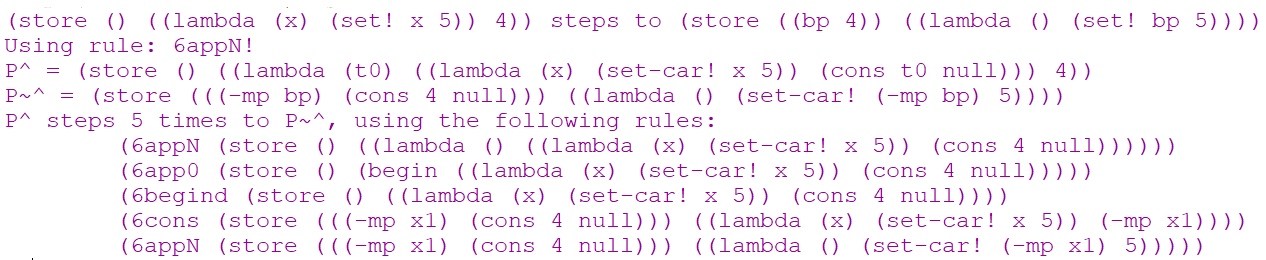
\includegraphics[ width=\textwidth]{figures/sim_example.PNG}
    \caption{Example of a Racket framework test case}
    \label{fig:rkt_sim_example}
\end{figure}

Figure \ref{fig:rkt_sim_example} is a text-based visualization of the process that our testing framework uses to validate our proof approach. In the full version of our test, we step until a limit is reached or no further steps are applicable and test the simulation relation for each step.

One very important detail of this framework can also be observed in figure \ref{fig:rkt_sim_example} --- that the terms we expect to match are not syntactically equivalent, but instead equal over $\alpha$-equivalence. To counteract this, in our test suites, we first normalize programs such that they are syntactically equal to all programs in their $\alpha$-equivalence class before comparing them. That way, we get positive results for comparing programs that are entirely the same except for a difference in naming. However, this also means that implicit shadowing or freshness of variables that have the same name is not allowed in this framework. Indeed, this makes it so that this framework does not typically mesh well with examples that include recursion, such as the Y-combinator.